\documentclass[11pt,a4paper]{article}

\usepackage[margin=1in]{geometry}
\usepackage[T1]{fontenc}
\usepackage{lmodern}
\usepackage{amsmath,amssymb}
\usepackage{graphicx}
\usepackage{booktabs}
\usepackage{array}
\usepackage{caption}
\usepackage{float}
\usepackage{enumitem}
\usepackage{algorithm}
\usepackage{algpseudocode}
\usepackage[hidelinks]{hyperref}

\graphicspath{{../results/figures/}}
\captionsetup{font=small,labelfont=bf}
\setlist{itemsep=2pt,topsep=4pt}

\hypersetup{
  pdftitle={Uncertainty for Optimal Memory Allocation},
  pdfauthor={Deval Singhal, Jayant Kumar, Sonal Mangesh Wagh, Sristi Vats, Shourya Veer Singh},
  pdfsubject={DA4022 Course Project 7 - Final Report}
}

\title{\textbf{Uncertainty for Optimal Memory Allocation}\\[4pt]
\large Uncertainty-Calibrated Allocation of KV-Cache Memory in\\Retrieval-Augmented Question Answering}

\author{
\begin{tabular}{ll}
Deval Singhal & 230101035 \\
Jayant Kumar & 230101050 \\
Sonal Mangesh Wagh & 230108054 \\
Sristi Vats & 230122057 \\
Shourya Veer Singh & 230106069 \\
\end{tabular}}

\date{DA4022 Course Project 7, Final Report\\[2pt] November 2026}

\begin{document}
\maketitle

\begin{abstract}
\noindent
The course question for this project is whether uncertainty can be used for
optimal memory allocation. We study it in retrieval-augmented question
answering, where the memory that grows with the input is the key-value (KV)
cache and the amount of retrieved text decides its size. Our method,
Uncertainty-Calibrated Allocation (UCA), starts every question with no
retrieved passages, reads the model's confidence, and adds passages only while
the model is still unsure. Confidence comes from the two assigned papers,
Internal Confidence and SemanticDPP, and from the probability the model assigns
to its own answer. We ran Qwen2.5-1.5B on 400 TriviaQA questions at five memory
levels on a laptop with 8\,GB of RAM. With at most two passages per question,
UCA matches the accuracy of giving every question two passages (57.6\% against
57.5\%) while holding 21\% less KV cache, and at very small budgets it is up to
7 accuracy points better than any allocation that ignores uncertainty. The
gain becomes small when memory is plentiful, and the method costs extra time.
We report both the positive results and the limits.
\end{abstract}

% ---------------------------------------------------------------------------
\section{Introduction}

A language model that answers questions with the help of retrieved text has to
keep that text in memory while it generates. The text is stored in the KV
cache, and the KV cache grows by a fixed number of bytes for every token in the
prompt. Systems normally retrieve the same number of passages for every
question. An easy question that the model already knows then occupies as much
memory as a hard one, and a hard one may still not get enough.

The two papers assigned to this project both measure how uncertain a model is.
Neither uses that measurement to decide how much memory a question should get.
This is the gap we work on. Our concrete question is:

\begin{quote}
\emph{How many retrieved passages should each question get when KV-cache memory is limited?}
\end{quote}

Our contributions are the following.
\begin{itemize}
\item A working implementation of both papers' uncertainty measures on a real
model, with Internal Confidence extended so that it can be read again after
passages have been added to the prompt.
\item UCA, a simple allocation policy with two settings: a confidence threshold
and a maximum number of passages. Confidence is first calibrated into a
probability of being correct, so that one threshold works for any signal.
\item An evaluation in actual KV-cache bytes against the strongest policy that
ignores uncertainty, together with the time cost of the confidence checks.
\item An honest account of what did not work, including our first design, which
decided the allocation once before retrieval.
\end{itemize}

% ---------------------------------------------------------------------------
\section{Background}

\subsection{The KV cache}

A transformer reads the prompt once and stores a key vector and a value vector
for every token in every layer. During generation it looks these up instead of
reading the prompt again. The size of this store is
\begin{equation}
\text{KV bytes} = N_{\text{tokens}} \times 2 \times L \times H_{\text{kv}} \times d_{\text{head}} \times b ,
\label{eq:kv}
\end{equation}
where $L$ is the number of layers, $H_{\text{kv}}$ the number of key-value
heads, $d_{\text{head}}$ the size of one head and $b$ the bytes per number. For
the model we use (Qwen2.5-1.5B in 16-bit floats, $L=28$, $H_{\text{kv}}=2$,
$d_{\text{head}}=128$, $b=2$) this gives 28{,}672 bytes per token. We compared
Equation~\ref{eq:kv} with the cache tensors returned by the model and the two
agree exactly. A prompt of 1{,}200 tokens therefore holds 34\,MB of KV cache.
This is per question: a server answering 64 questions at the same time needs
2.2\,GB of KV cache for a model whose weights take 3.1\,GB.

\subsection{Retrieval and the memory knob}

In retrieval-augmented generation the system finds passages related to the
question and places them in the prompt. More passages make it more likely that
the answer is present, and they enlarge the KV cache in proportion. In this
setting the memory given to a question is set by the number of passages in its
prompt. We use five levels: 0, 1, 2, 4 and 8 passages.

\subsection{Judging an uncertainty score}

An uncertainty score is useful if it is high for answers that turn out wrong
and low for answers that turn out right. We measure this with the area under
the ROC curve (AUROC), as both papers do. It is the probability that a randomly
chosen wrong answer receives a higher uncertainty than a randomly chosen right
one; 0.5 means the score carries no information and 1.0 is perfect.

% ---------------------------------------------------------------------------
\section{The Two Reference Papers}

\subsection{Internal Confidence (Chen et al., ICLR 2026)}

Chen et al.~\cite{chen2026query} estimate uncertainty before any text is
generated. The model is given the prompt ``Respond only with `Yes' or `No' to
indicate whether you are capable of answering the following question
accurately.'' For the hidden state $h_n^{(l)}$ at layer $l$ and token $n$, the
probability of ``Yes'' is obtained by projecting onto the output embeddings of
the two tokens:
\begin{equation}
P(\text{Yes}\mid h_n^{(l)}) = \operatorname{softmax}\bigl(W^{\text{unemb}}_{[\text{Yes},\text{No}]}\, h_n^{(l)}\bigr)_{\text{Yes}} .
\end{equation}
The Internal Confidence (IC) is a weighted sum over layers and over the last
few tokens,
\begin{equation}
\mathrm{IC} = \sum_{n}\sum_{l} w_n\, w_l\; P(\text{Yes}\mid h_n^{(l)}),
\qquad
w_j = \frac{\exp(-\alpha\,|i-j|^2)}{\sum_{j'}\exp(-\alpha\,|i-j'|^2)},
\end{equation}
where $i$ is the last layer (or last token) and $\alpha = 1$. With this choice
the last position receives about 72\% of the weight and its neighbour about
27\%. The method needs one forward pass and no training. In the paper it is
used for one decision made before retrieval: retrieve or do not retrieve.

\subsection{SemanticDPP (anonymous, under review at ICLR 2026)}

SemanticDPP~\cite{semanticdpp2026} measures uncertainty from several sampled
answers to the same question. Each answer is represented by the last-layer
hidden state of the generating model, averaged over the answer's tokens. A
small network $\phi$ maps these embeddings to a space in which distance
reflects difference in meaning, and a kernel is defined on that space:
\begin{equation}
L_{ij} = \exp\bigl(-\alpha\,\lVert \phi(x_i)-\phi(x_j)\rVert^2\bigr).
\end{equation}
The network is trained by maximising the likelihood of a determinantal point
process (DPP), $\log\det(L_Y) - \log\det(L+I)$, where $Y$ contains one answer
from each group of answers with the same meaning. The uncertainty of a set $S$
of sampled answers is
\begin{equation}
U(S) = \log\det K_S, \qquad K = L\,(L+I)^{-1}.
\end{equation}
Answers that all mean the same give a strongly negative value; answers that
differ give a larger one. In the paper the score is used to decide whether the
model should abstain.

\subsection{What the papers leave open}

Both papers stop at the uncertainty number. Internal Confidence is cheap but is
read only once, before any memory has been given. SemanticDPP is more
informative but needs several sampled answers. Neither connects the score to
the amount of memory a question should receive.

% ---------------------------------------------------------------------------
\section{Method: Uncertainty-Calibrated Allocation}

\subsection{Idea}

A student in an open-book exam answers an easy question from memory. If unsure,
the student opens one page and tries again, and reads further only while still
unsure. UCA applies the same procedure to a language model
(Algorithm~\ref{alg:uca}). Every question starts with no passages. After each
attempt the model's confidence is read. If it is high enough the answer is
kept; otherwise more passages are added. The KV-cache memory used by a question
is the memory of the level at which it stops.

\begin{algorithm}[H]
\caption{Uncertainty-Calibrated Allocation for one question}
\label{alg:uca}
\begin{algorithmic}[1]
\Require question $q$, ranked passages, levels $k_0<k_1<\dots<k_m$ (here $0,1,2,4,8$),
threshold $\tau$, maximum level $k_{\max}$, calibration curves $g_0,\dots,g_{m-1}$
\For{$c = 0,1,\dots,m$}
  \State answer $q$ with the top $k_c$ passages in the prompt
  \If{$k_c = k_{\max}$} \Return the answer \EndIf
  \State read the confidence score $s_c$
  \State $p \gets g_c(s_c)$ \Comment{calibrated probability that the answer is correct}
  \If{$p \ge \tau$} \Return the answer \EndIf
\EndFor
\end{algorithmic}
\end{algorithm}

The policy has two settings. The threshold $\tau$ says how sure is sure enough:
a low value saves more memory and risks some accuracy. The maximum level bounds
the memory any single question can take.

\subsection{Calibration}

Raw confidence scores are on different scales. An Internal Confidence of 0.6, a
log-probability of $-0.4$ and a DPP score of $-20$ cannot be compared with each
other or with a threshold. For each signal and each memory level we therefore
fit a monotone step function (isotonic regression) on held-out questions that
maps a score to the fraction of answers with that score that were correct.
After calibration, ``stop when $p \ge 0.7$'' has the same meaning for every
signal.

\subsection{Confidence signals}

We use four signals inside the same policy.
\begin{itemize}
\item \textbf{Internal Confidence.} Paper~\cite{chen2026query}, read again at
every level with the current passages placed before the self-assessment
question. Re-reading it with context is our extension. Cost per check: one
forward pass, no generation.
\item \textbf{SemanticDPP.} Paper~\cite{semanticdpp2026}, computed on five
sampled answers at every level. Cost per check: five short sampled answers.
\item \textbf{Answer probability.} The probability the model assigns to its own
greedy answer (the sum of the log-probabilities of the generated tokens). It is
a standard baseline, listed as maximum sequence probability
in~\cite{chen2026query}, and it comes with the answer at no extra cost.
\item \textbf{All three combined.} The average of the three calibrated
probabilities.
\end{itemize}

\subsection{What we compare against}

\begin{itemize}
\item \textbf{Same memory for everyone.} Every question gets $k$ passages. We
also allow the best random mix of two such settings, for example 60\% of the
questions with one passage and 40\% with two, so that any average memory can be
met. This is the strongest policy that does not look at uncertainty.
\item \textbf{Deciding once, before retrieval.} The confidence without passages
is read one time and the number of passages is assigned from that single value,
using a table of expected accuracy per confidence bin and a greedy budget
split. This follows the adaptive-retrieval use in~\cite{chen2026query} and was
our own first design.
\item \textbf{Oracle.} A reference that knows the correct answers and gives
each question the cheapest level at which it is answered correctly. It cannot
be built in practice and only shows how much room there is.
\end{itemize}

% ---------------------------------------------------------------------------
\section{Experimental Setup}

\begin{table}[H]
\centering
\small
\begin{tabular}{@{}p{3.2cm}p{11cm}@{}}
\toprule
Model & Qwen2.5-1.5B-Instruct, 16-bit floats \\
Hardware & Apple M1 laptop, 8\,GB RAM, model on the integrated GPU \\
Data & 400 questions from the TriviaQA validation set~\cite{joshi2017triviaqa}, which both papers use \\
Retrieval & Wikipedia evidence pages of each question, cut into 100-word passages and ranked with BM25 \\
Memory levels & 0, 1, 2, 4, 8 passages, about 51, 199, 343, 629 and 1{,}200 prompt tokens \\
Correctness & the answer contains one of the accepted TriviaQA aliases after lower-casing and removing punctuation \\
SemanticDPP & 5 samples, temperature 1.0, top-$p$ 0.9; kernel trained on calibration questions \\
Evaluation & fitted on 200 questions and tested on the other 200, repeated for 20 random halvings \\
\bottomrule
\end{tabular}
\caption{Experimental setup.}
\label{tab:setup}
\end{table}

The model was run once on every question at every level, and the answers,
timings and confidence signals were saved. Any allocation policy can then be
evaluated exactly by looking up the saved answers. Everything that is fitted
(the calibration curves and the DPP kernel) uses only the calibration half of a
split. We report the mean over the 20 halvings and, after the $\pm$ sign, the
standard deviation over them.

\paragraph{Differences from the papers.} For Internal Confidence we read the
intermediate layers through the model's final normalisation layer before
projecting onto the output embeddings. For SemanticDPP the paper obtains its
training labels from an entailment model; TriviaQA answers are a few words
long, so we group sampled answers by normalised string match instead. We also
whiten the embeddings with a 32-dimensional PCA because we have only a few
hundred calibration questions.

\paragraph{Two implementation points on small hardware.} First, a direct
implementation samples five answers by running the prompt five times in a
batch, which also keeps five copies of the prompt's KV cache. We read the
prompt once and decode all five samples from the same cached keys and values.
With four passages in the prompt this reduced the sampling time from about
7\,s to about 1.4\,s in our tests, and sampling no longer multiplies the prompt
memory. Second, the GPU memory cache has to be released after every question;
otherwise memory use kept growing on the 8\,GB machine and the time per
question roughly doubled.

% ---------------------------------------------------------------------------
\section{Results}

\subsection{The effect of memory alone}

\begin{table}[H]
\centering
\small
\begin{tabular}{@{}rrrrr@{}}
\toprule
Passages for every question & Accuracy & Prompt tokens & KV cache per question & Time per question \\
\midrule
0 & 32.1\% & 51 & 1.5\,MB & 0.46\,s \\
1 & 52.0\% & 199 & 5.7\,MB & 0.70\,s \\
2 & 57.5\% & 343 & 9.8\,MB & 1.05\,s \\
4 & 62.6\% & 629 & 18.0\,MB & 1.70\,s \\
8 & 65.9\% & 1{,}200 & 34.4\,MB & 3.37\,s \\
\bottomrule
\end{tabular}
\caption{Accuracy and cost when every question receives the same number of passages.}
\label{tab:fixed}
\end{table}

Table~\ref{tab:fixed} shows that going from two to eight passages costs 3.5
times the memory for about 8 points of accuracy. The averages hide three facts.
Of the questions answered correctly without passages, only 75\% remain correct
when one passage is added, and 82\% with eight: retrieved text can distract the
model from something it already knew. Of the questions answered wrongly without
passages, 41\% are corrected by one passage and 59\% by eight. Finally, 77.5\%
of the questions are answered correctly at some level, although the best single
level reaches only 65.9\%; the oracle reaches 77.4\% with 5.7\,MB per question.
There is therefore a large gain available from giving each question the right
amount. The remaining sections ask how much of it uncertainty can recover.

\subsection{Quality of the confidence signals}

\begin{table}[H]
\centering
\small
\begin{tabular}{@{}lcccc@{}}
\toprule
 & \multicolumn{4}{c}{Passages in the prompt} \\
\cmidrule(l){2-5}
Confidence signal & 0 & 1 & 2 & 4 \\
\midrule
Internal Confidence~\cite{chen2026query} & 0.64 & 0.74 & 0.75 & 0.75 \\
\quad P(Yes), last layer and token only & 0.60 & 0.73 & 0.75 & 0.75 \\
\quad P(Yes), plain average & 0.67 & 0.73 & 0.73 & 0.75 \\
SemanticDPP~\cite{semanticdpp2026} & 0.83 & 0.74 & 0.73 & 0.71 \\
\quad untrained kernel & 0.83 & 0.74 & 0.73 & 0.71 \\
\quad sampled answers agree (string match) & 0.84 & 0.74 & 0.72 & 0.71 \\
Answer probability & 0.87 & 0.78 & 0.77 & 0.79 \\
\bottomrule
\end{tabular}
\caption{AUROC for separating correct from incorrect answers on held-out
questions. The standard deviation over the 20 halvings is between 0.01 and
0.03 for every entry.}
\label{tab:auroc}
\end{table}

\begin{figure}[H]
\centering
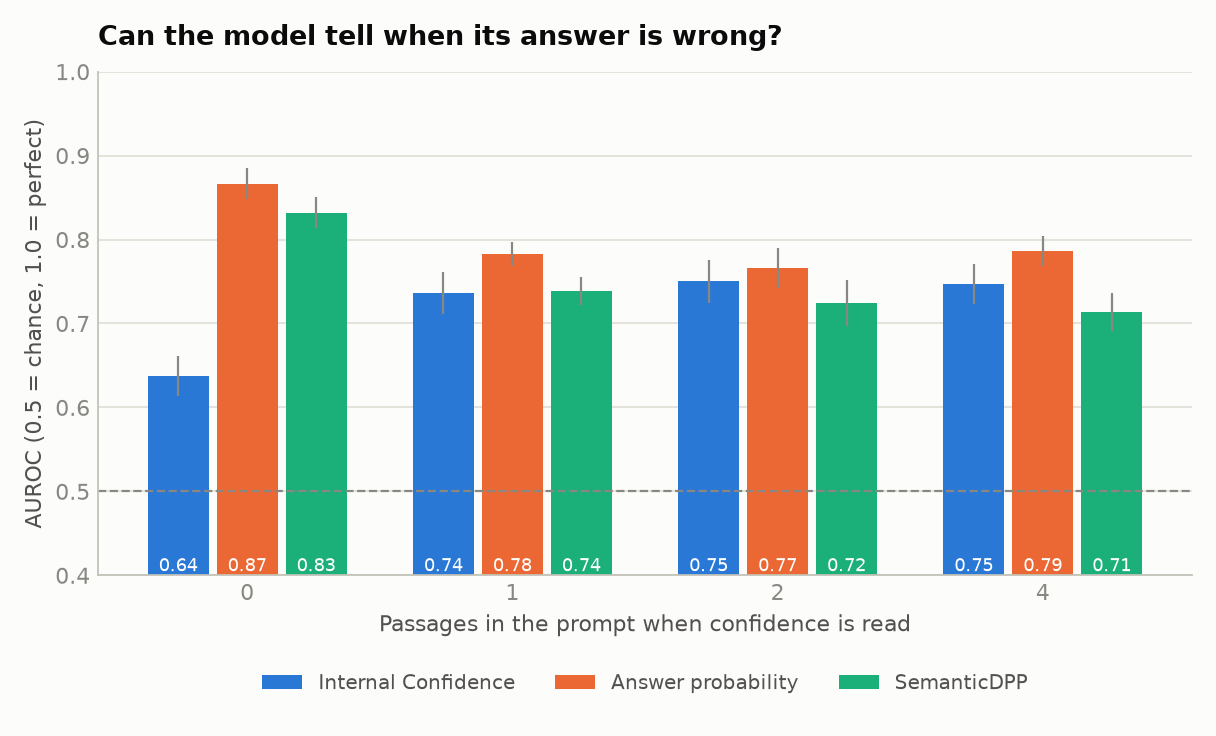
\includegraphics[width=0.78\linewidth]{signal_quality.png}
\caption{AUROC of the three main signals at each memory level.}
\label{fig:quality}
\end{figure}

Table~\ref{tab:auroc} and Figure~\ref{fig:quality} give four observations.

\emph{Our Internal Confidence result agrees with the paper.} Without passages
we obtain 0.64. Chen et al.\ report 0.647 on TriviaQA for their smallest model
(Phi-3, 3.8B parameters) and up to 0.719 for a 14B model. Our model is smaller
than any of theirs.

\emph{Internal Confidence improves once passages are present} (0.64 to 0.75).
Whether the available text is enough to answer appears to be easier for the
model to judge than whether it knows the answer by itself.

\emph{The answer-based signals are strongest before retrieval} (0.83 to 0.87)
and fall to 0.71--0.79 with passages. With passages the sampled answers agree
much more often: on average 3.1 different answers out of five without
passages, and 1.5 with four. They also agree when the answer has been copied
from a misleading passage, which hides the error from these signals.

\emph{The trained DPP kernel did not help in our setting.} It is no better than
an untrained kernel, and counting how many sampled answers match as strings
performs equally well. TriviaQA answers are one or two words, so there is
little difference between ``same meaning'' and ``same string'' for the DPP to
resolve, and our kernel is trained on only 200 questions with string-match
labels. We did not test longer answers, where this may be different.

\begin{figure}[H]
\centering
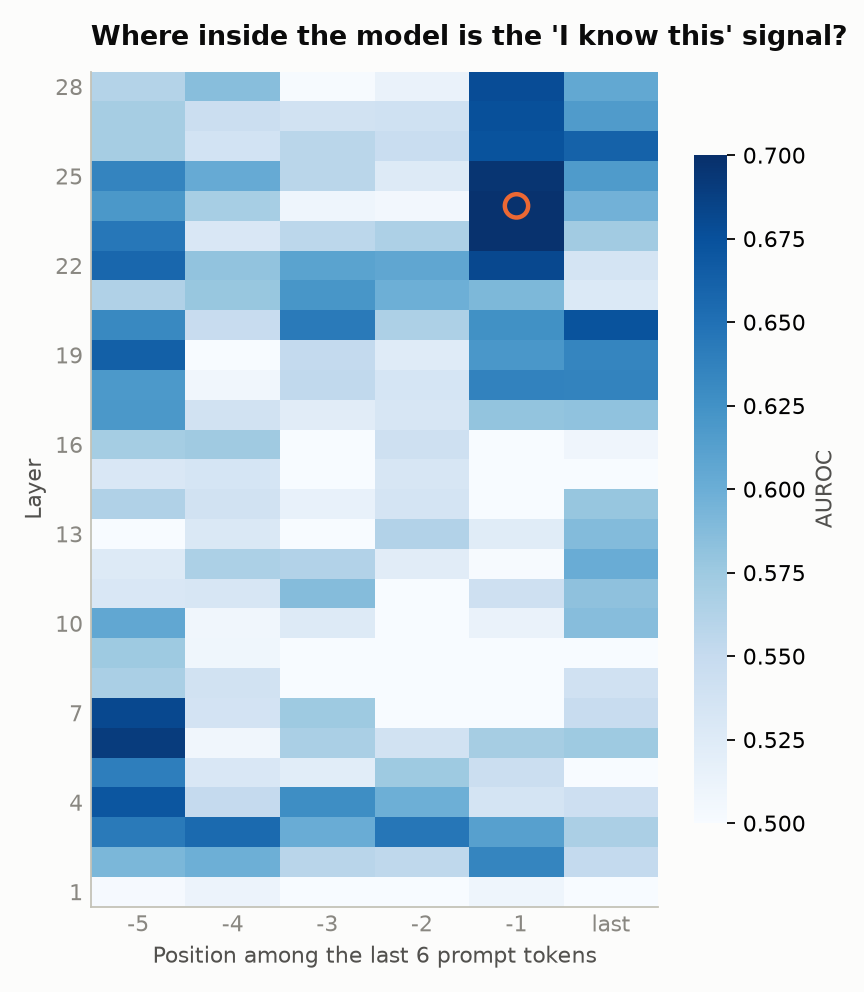
\includegraphics[width=0.42\linewidth]{ic_heatmap.png}
\caption{AUROC of P(Yes) at each layer and each of the last six prompt tokens,
without passages. The circle marks the best cell.}
\label{fig:heatmap}
\end{figure}

Figure~\ref{fig:heatmap} shows where the self-assessment signal lies inside the
model. Chen et al.\ observe that the most informative position is not
necessarily the last layer and last token. We see the same: the best single
cell is layer 24 of 28, one token before the end (AUROC 0.70), against 0.61 at
the final cell.

\subsection{Memory saved by UCA}

\begin{figure}[H]
\centering
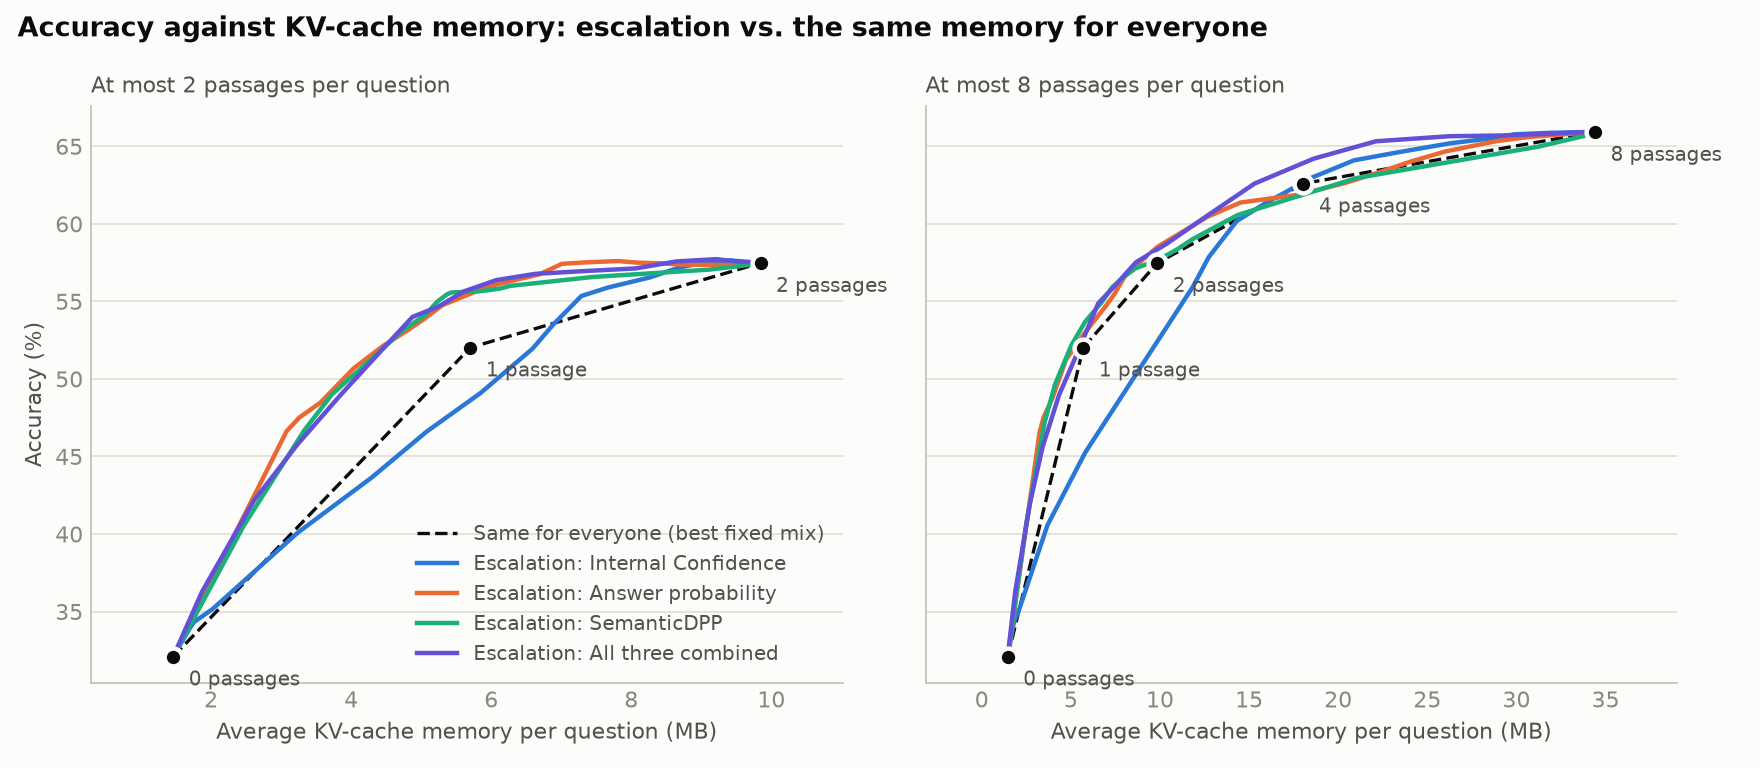
\includegraphics[width=\linewidth]{accuracy_vs_memory.png}
\caption{Accuracy against average KV-cache memory per question. Each coloured
line is UCA with one confidence signal as the threshold moves from ``always
stop'' (left end) to ``never stop early'' (right end). Black dots give every
question the same number of passages; the dashed line joining them is the best
policy that ignores uncertainty. Left: at most two passages. Right: at most
eight.}
\label{fig:main}
\end{figure}

Figure~\ref{fig:main} is the main result. A coloured line above the dashed line
means more accuracy from the same KV-cache memory. Table~\ref{tab:headline}
gives the same information at one fixed threshold, $\tau = 0.70$.

\begin{table}[H]
\centering
\small
\begin{tabular}{@{}lrrrrrr@{}}
\toprule
Confidence signal & Accuracy & KV cache & Memory & Accuracy & Gain over blind mix & Time \\
 & & & saved & change & at equal memory & \\
\midrule
\multicolumn{7}{@{}l}{\emph{At most 2 passages. Every question gets 2: 57.5\%, 9.8\,MB, 1.05\,s}} \\
Answer probability & 57.6\% & 7.8\,MB & 21\% & $+0.1 \pm 0.8$ & $+2.6 \pm 1.0$ & 1.75\,s \\
SemanticDPP & 56.6\% & 7.4\,MB & 24\% & $-0.9 \pm 1.2$ & $+2.2 \pm 1.8$ & 4.29\,s \\
Internal Confidence & 57.2\% & 8.7\,MB & 12\% & $-0.3 \pm 0.7$ & $+1.0 \pm 0.9$ & 1.72\,s \\
All three combined & 57.6\% & 8.6\,MB & 12\% & $+0.1 \pm 0.6$ & $+1.5 \pm 1.1$ & 5.51\,s \\
\midrule
\multicolumn{7}{@{}l}{\emph{At most 8 passages. Every question gets 8: 65.9\%, 34.4\,MB, 3.37\,s}} \\
All three combined & 65.3\% & 22.1\,MB & 36\% & $-0.6 \pm 1.1$ & $+1.9 \pm 1.5$ & 12.05\,s \\
Internal Confidence & 64.1\% & 20.9\,MB & 39\% & $-1.8 \pm 1.8$ & $+0.9 \pm 1.5$ & 4.38\,s \\
Answer probability & 62.6\% & 20.4\,MB & 41\% & $-3.3 \pm 1.5$ & $-0.4 \pm 1.3$ & 4.36\,s \\
SemanticDPP & 60.6\% & 14.4\,MB & 58\% & $-5.4 \pm 2.3$ & $+0.2 \pm 1.4$ & 7.22\,s \\
\bottomrule
\end{tabular}
\caption{UCA at threshold 0.70. ``Accuracy change'' is against giving every
question the maximum number of passages. ``Gain over blind mix'' is against
the best uncertainty-blind policy that uses the same average memory. Both are
in accuracy points.}
\label{tab:headline}
\end{table}

\paragraph{Small memory ceiling.} With at most two passages and answer
probability as the signal, UCA matches the accuracy of giving everyone two
passages (57.6\% against 57.5\%) with 21\% less KV cache. At a slightly lower
threshold of 0.60 the saving is 29\% at the same accuracy (57.4\% with
7.0\,MB).

\paragraph{Smallest budgets.} The largest gains are at the low end. With answer
probability, at most one passage and a threshold of 0.25, UCA reaches 48.8\%
with 3.5\,MB, which is $7.2 \pm 1.8$ points above the best blind policy at that
memory. At about the memory of one passage for everyone (5.7\,MB, 52.0\%),
escalation up to two passages reaches 56.0\% with 5.9\,MB, a gain of
$4.0 \pm 1.5$ points at equal memory. In this range the decision is mostly
whether a question needs retrieval at all, and the model judges that well
(AUROC 0.87).

\paragraph{Large memory ceiling.} With at most eight passages UCA saves between
36\% and 58\% of the memory but loses between 1 and 5 points of accuracy.
Against the best blind mix at the same memory it is about level ($-0.4$ to
$+1.9$ points, comparable to the noise). Only the combination of the three
signals stays close to the full accuracy, 65.3\% against 65.9\%, with 36\% less
memory.

\paragraph{Internal Confidence alone.} It is the weakest of the three signals
on this model, with a gain of about one point. It contributes in the
combination, and the paper reports that it improves with model size, which we
could not test on our hardware.

\begin{figure}[H]
\centering
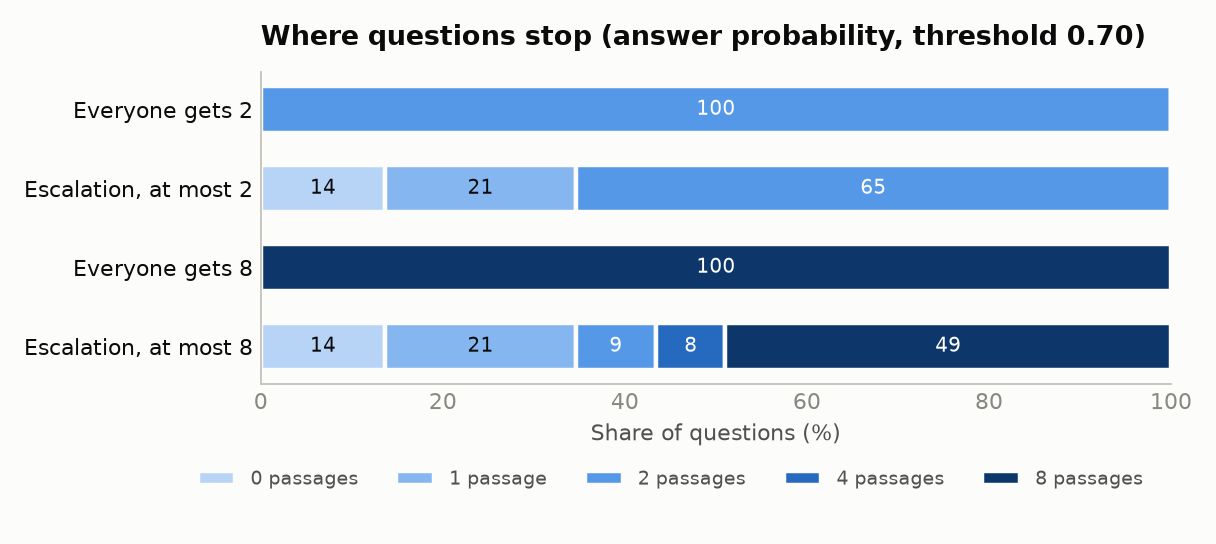
\includegraphics[width=0.8\linewidth]{where_questions_stop.png}
\caption{Share of questions ending at each memory level, for UCA with answer
probability at threshold 0.70, next to the corresponding fixed settings.}
\label{fig:stop}
\end{figure}

Figure~\ref{fig:stop} shows where the saving comes from: 14\% of the questions
stop without any passage and a further 21\% after one.

\subsection{Deciding once before retrieval}

Our first design read the confidence without passages one time and assigned the
number of passages from it. Averaged over all memory budgets, its gain over the
best blind mix was $+0.3 \pm 1.0$ points with Internal Confidence and
$0.0 \pm 1.3$ points with a cascade that calls SemanticDPP only when Internal
Confidence is in its middle range. Neither is distinguishable from zero. The
reason is that about two thirds of the questions are wrong without passages and
need retrieval in any case, and the confidence measured without passages says
nothing about how many passages will be enough. Confidence has to be read again
after memory has been given, which is what led us to the escalation design.

\subsection{Cost of the confidence checks}

\begin{table}[H]
\centering
\small
\begin{tabular}{@{}lcccc@{}}
\toprule
 & \multicolumn{4}{c}{Passages already in the prompt} \\
\cmidrule(l){2-5}
Check & 0 & 1 & 2 & 4 \\
\midrule
Internal Confidence (one forward pass) & 0.25\,s & 0.53\,s & 0.86\,s & 1.51\,s \\
SemanticDPP (5 samples from the shared cache) & 1.51\,s & 1.39\,s & 1.50\,s & 1.54\,s \\
Answer probability & 0 & 0 & 0 & 0 \\
\bottomrule
\end{tabular}
\caption{Median time of one confidence check on the M1 laptop.}
\label{tab:time}
\end{table}

UCA saves memory and not time. Each further level reads a longer prompt again.
With at most two passages the answer-probability policy takes 1.75\,s per
question against 1.05\,s for giving everyone two passages: 21\% less memory for
67\% more time. SemanticDPP costs about four times the time. Internal
Confidence is cheap in the paper because it generates nothing, but once
passages are in the prompt it has to read them as well, and its prompt is about
32 tokens longer than the answering prompt. Peak memory is not affected by the
checks, since each check finishes before the next level starts.

Most of the additional time could be avoided. When moving from one passage to
two, the first passage is unchanged, and its cached keys and values could be
kept rather than recomputed. We did not implement this.

% ---------------------------------------------------------------------------
\section{Discussion and Limitations}

\paragraph{What we learned.}
\begin{enumerate}
\item Uncertainty is most useful for the first decision, namely whether a
question needs any retrieved memory. There the gain is clear.
\item Uncertainty does not identify questions that no amount of memory will
fix. About 22\% of the questions are wrong at every level. They look unsure all
the way up, so an uncertainty-driven policy keeps giving them memory that does
not pay off. The oracle avoids this and none of our signals can. This is the
main reason the gain shrinks at large budgets.
\item The cheapest signal was the best. The probability of the model's own
answer did better than both papers' methods on this task and costs nothing.
\item Simple policies generalised and more elaborate ones did not. We also
tried a rule based on expected accuracy gain per extra token, and thresholds
tuned separately for every budget. Both looked better on calibration questions
and worse on test questions. With a few hundred questions to calibrate on, two
settings were all we could choose reliably.
\end{enumerate}

\paragraph{Limitations.}
\begin{itemize}
\item We used one small model, one dataset and 400 questions. The values after
$\pm$ are the spread over random halvings of the same questions and therefore
understate the true uncertainty. Differences of about one point should be read
as no difference; the gains of 2 to 7 points at small budgets are the ones we
rely on.
\item The threshold of 0.70 in Table~\ref{tab:headline} and the form of the
policy were fixed after looking at the first 200 questions. The full curves in
Figure~\ref{fig:main} do not depend on that choice.
\item Correctness is decided by string matching against TriviaQA aliases, which
is strict about wording and occasionally lenient for very short aliases.
\item Retrieval uses BM25 over the evidence pages of each question, which is
easier than searching all of Wikipedia.
\item Time increases with our implementation, as shown in Table~\ref{tab:time}.
\end{itemize}

% ---------------------------------------------------------------------------
\section{Changes Since the Mid-Term Report}

The mid-term report described a design called Uncertainty-Calibrated Adaptive
Compression and quoted AUROC values of 92\% and 100\%. Those values came from a
simulation in which the uncertainty scores and the correctness labels were
generated from the same difficulty tag; they were not measurements of a model
and they are replaced by the results in this report. When we moved to a real
model we also changed the design:
\begin{itemize}
\item The mapping from DPP eigenvalues to per-dimension compression ratios was
dropped. The eigenvalues describe how a handful of sampled answers differ from
each other and do not correspond to dimensions of the KV cache.
\item The hand-set formula for the KV budget and the beam-width control were
replaced by a memory setting that is actually applied (the number of passages)
and measured in bytes.
\item The plan of running Internal Confidence first and SemanticDPP only for
uncertain questions was kept and tested as the one-shot cascade of Section~6.4.
It gave no gain, for the reason explained there.
\item The model was changed from Llama-3.2-3B to Qwen2.5-1.5B so that all
experiments run on an 8\,GB laptop.
\end{itemize}

% ---------------------------------------------------------------------------
\section{Conclusion and Future Work}

We asked whether uncertainty can guide the allocation of KV-cache memory and
tested it on a real model with exact memory accounting. Reading the model's
confidence after each increase in memory, and stopping as soon as it is high
enough, gives the same accuracy as a fixed two-passage setting with 21\% less
KV cache, and up to 7 points more accuracy than uncertainty-blind allocation at
very small budgets. The benefit fades when memory is plentiful, and it is paid
for in time. Deciding the allocation once before retrieval did not help.

Four extensions follow directly from the limits we found.
\begin{itemize}
\item \textbf{Reuse the KV cache between escalation steps.} If passages are
placed before the question so that adding one only appends to the prompt, the
cached part can be kept and only the new tokens computed. This should remove
most of the time overhead.
\item \textbf{A larger model.} Chen et al.\ show Internal Confidence improving
with model size. A 7--8B model on a GPU machine would show whether the
pre-generation signal becomes competitive.
\item \textbf{Detecting questions that retrieval cannot help}, for instance by
checking whether the retrieved passages are relevant at all, so that memory is
not spent where it has no effect.
\item \textbf{Longer answers}, where the meaning-based comparison of SemanticDPP
should matter more than it does for one-word answers.
\end{itemize}

% ---------------------------------------------------------------------------
\begin{thebibliography}{9}

\bibitem{chen2026query}
L.~Chen, G.~de~Melo, F.~M.~Suchanek, and G.~Varoquaux.
\newblock Query-level uncertainty in large language models.
\newblock In \emph{International Conference on Learning Representations (ICLR)}, 2026.
\newblock \url{https://openreview.net/pdf?id=11QZITAMUO}

\bibitem{semanticdpp2026}
Anonymous.
\newblock SemanticDPP: Efficient uncertainty quantification in LLMs.
\newblock Under review at the \emph{International Conference on Learning Representations (ICLR)}, 2026.
\newblock \url{https://openreview.net/pdf?id=C8yjlrx4Wo}

\bibitem{joshi2017triviaqa}
M.~Joshi, E.~Choi, D.~S.~Weld, and L.~Zettlemoyer.
\newblock TriviaQA: A large scale distantly supervised challenge dataset for reading comprehension.
\newblock In \emph{Proceedings of the 55th Annual Meeting of the Association for Computational Linguistics (ACL)}, 2017.

\end{thebibliography}

% ---------------------------------------------------------------------------
\appendix
\section{Reproducing the Results}

The code is at \url{https://github.com/maidevalhoon/DA4022}. All commands are
run from the repository root with Python 3.11.

\begin{table}[H]
\centering
\small
\begin{tabular}{@{}p{7.4cm}p{7.2cm}@{}}
\toprule
Command & Purpose \\
\midrule
\texttt{python -m pytest tests -q} & unit tests for the weights, the DPP, the allocation policies and the metrics \\
\texttt{python -m src.experiments.prepare\_data} & builds the TriviaQA subset with retrieved passages \\
\texttt{python -m src.experiments.collect} & runs the model on 400 questions at every memory level (about two hours on the M1; resumable) \\
\texttt{python -m src.experiments.analyze} & computes every table and figure in this report from the saved runs \\
\texttt{python -m src.experiments.demo -{}-n 10} & live run on questions that were not used in the experiments \\
\bottomrule
\end{tabular}
\caption{Commands.}
\end{table}

The saved model runs (\texttt{results/runs.jsonl}, \texttt{results/runs.npz})
are included in the repository, so the analysis can be repeated without
running the model.

\end{document}
